\documentclass[12pt,a4paper]{article}

%\usepackage[left=1.5cm,right=1.5cm,top=1cm,bottom=2cm]{geometry}
\usepackage[in, plain]{fullpage}
\usepackage{array}
\usepackage{../../../pas-math}
\usepackage{../../../moncours}


%\usepackage{pas-cours}
%-------------------------------------------------------------------------------
%          -Packages nécessaires pour écrire en Français et en UTF8-
%-------------------------------------------------------------------------------
\usepackage[utf8]{inputenc}
\usepackage[frenchb]{babel}
\usepackage[T1]{fontenc}
\usepackage{lmodern}
\usepackage{textcomp}



%-------------------------------------------------------------------------------

%-------------------------------------------------------------------------------
%                          -Outils de mise en forme-
%-------------------------------------------------------------------------------
\usepackage{hyperref}
\hypersetup{pdfstartview=XYZ}
%\usepackage{enumerate}
\usepackage{graphicx}
\usepackage{multicol}
\usepackage{tabularx}
\usepackage{multirow}


\usepackage{anysize} %%pour pouvoir mettre les marges qu'on veut
%\marginsize{2.5cm}{2.5cm}{2.5cm}{2.5cm}

\usepackage{indentfirst} %%pour que les premier paragraphes soient aussi indentés
\usepackage{verbatim}
\usepackage{enumitem}
\usepackage[usenames,dvipsnames,svgnames,table]{xcolor}

\usepackage{variations}

%-------------------------------------------------------------------------------


%-------------------------------------------------------------------------------
%                  -Nécessaires pour écrire des mathématiques-
%-------------------------------------------------------------------------------
\usepackage{amsfonts}
\usepackage{amssymb}
\usepackage{amsmath}
\usepackage{amsthm}
\usepackage{tikz}
\usepackage{xlop}
%-------------------------------------------------------------------------------



%-------------------------------------------------------------------------------


%-------------------------------------------------------------------------------
%                    - Mise en forme avancée
%-------------------------------------------------------------------------------

\usepackage{ifthen}
\usepackage{ifmtarg}


\newcommand{\ifTrue}[2]{\ifthenelse{\equal{#1}{true}}{#2}{$\qquad \qquad$}}

%-------------------------------------------------------------------------------

%-------------------------------------------------------------------------------
%                     -Mise en forme d'exercices-
%-------------------------------------------------------------------------------
%\newtheoremstyle{exostyle}
%{\topsep}% espace avant
%{\topsep}% espace apres
%{}% Police utilisee par le style de thm
%{}% Indentation (vide = aucune, \parindent = indentation paragraphe)
%{\bfseries}% Police du titre de thm
%{.}% Signe de ponctuation apres le titre du thm
%{ }% Espace apres le titre du thm (\newline = linebreak)
%{\thmname{#1}\thmnumber{ #2}\thmnote{. \normalfont{\textit{#3}}}}% composants du titre du thm : \thmname = nom du thm, \thmnumber = numéro du thm, \thmnote = sous-titre du thm

%\theoremstyle{exostyle}
%\newtheorem{exercice}{Exercice}
%
%\newenvironment{questions}{
%\begin{enumerate}[\hspace{12pt}\bfseries\itshape a.]}{\end{enumerate}
%} %mettre un 1 à la place du a si on veut des numéros au lieu de lettres pour les questions 
%-------------------------------------------------------------------------------

%-------------------------------------------------------------------------------
%                    - Mise en forme de tableaux -
%-------------------------------------------------------------------------------

\renewcommand{\arraystretch}{1.7}

\setlength{\tabcolsep}{1.2cm}

%-------------------------------------------------------------------------------



%-------------------------------------------------------------------------------
%                    - Racourcis d'écriture -
%-------------------------------------------------------------------------------

% Angles orientés (couples de vecteurs)
\newcommand{\aopp}[2]{(\vec{#1}, \vec{#2})} %Les deuc vecteurs sont positifs
\newcommand{\aopn}[2]{(\vec{#1}, -\vec{#2})} %Le second vecteur est négatif
\newcommand{\aonp}[2]{(-\vec{#1}, \vec{#2})} %Le premier vecteur est négatif
\newcommand{\aonn}[2]{(-\vec{#1}, -\vec{#2})} %Les deux vecteurs sont négatifs

%Ensembles mathématiques
\newcommand{\naturels}{\mathbb{N}} %Nombres naturels
\newcommand{\relatifs}{\mathbb{Z}} %Nombres relatifs
\newcommand{\rationnels}{\mathbb{Q}} %Nombres rationnels
\newcommand{\reels}{\mathbb{R}} %Nombres réels
\newcommand{\complexes}{\mathbb{C}} %Nombres complexes


%Intégration des parenthèses aux cosinus
\newcommand{\cosP}[1]{\cos\left(#1\right)}
\newcommand{\sinP}[1]{\sin\left(#1\right)}


%Probas stats
\newcommand{\stat}{statistique}
\newcommand{\stats}{statistiques}
%-------------------------------------------------------------------------------

%-------------------------------------------------------------------------------
%                    - Mise en page -
%-------------------------------------------------------------------------------

\newcommand{\twoCol}[1]{\begin{multicols}{2}#1\end{multicols}}


\setenumerate[1]{font=\bfseries,label=\textit{\alph*})}
\setenumerate[2]{font=\bfseries,label=\arabic*)}


%-------------------------------------------------------------------------------
%                    - Elements cours -
%-------------------------------------------------------------------------------





%\makeatletter
%\renewcommand*{\@seccntformat}[1]{\csname the#1\endcsname\hspace{0.1cm}}
%\makeatother


%\author{Olivier FINOT}
\date{}
\title{}

%\newcommand{\disp}{false}

%
%\rfoot{Page \thepage}
\begin{document}
%\maketitle
\chap[num=2, color=red]{Fonctions de référence}{Olivier FINOT, \today }

\section{Rappels}



\begin{mydefs}
	
	\begin{itemize}
		\item Toute fonction est définie sur \kw{intervalle} I.
		
		\item Elle a un nom, souvent \kw{$f$}.
		
		\item Le nombre de départ, \kw{la variable} est en général appelé $x$. Le nombre qui lui est associé est alors noté \kw{$f(x)$}.
		
		\item Le nombre $f(x)$ est appelé \kw{image de $x$} par la fonction $f$.
		
		\item \kw{x} est appelé \kw{antécédentde $f(x)$} par la fonction $f$
		
		\item $f$ est \kw{croissante} si $f(x)$ augmente quand $x$ augmente.
		
		\item $f$ est \kw{décroissante} si $f(x)$ diminue quand $x$ augmente.
	\end{itemize}
	
	%

\end{mydefs}

\begin{myillus}
	{\centering 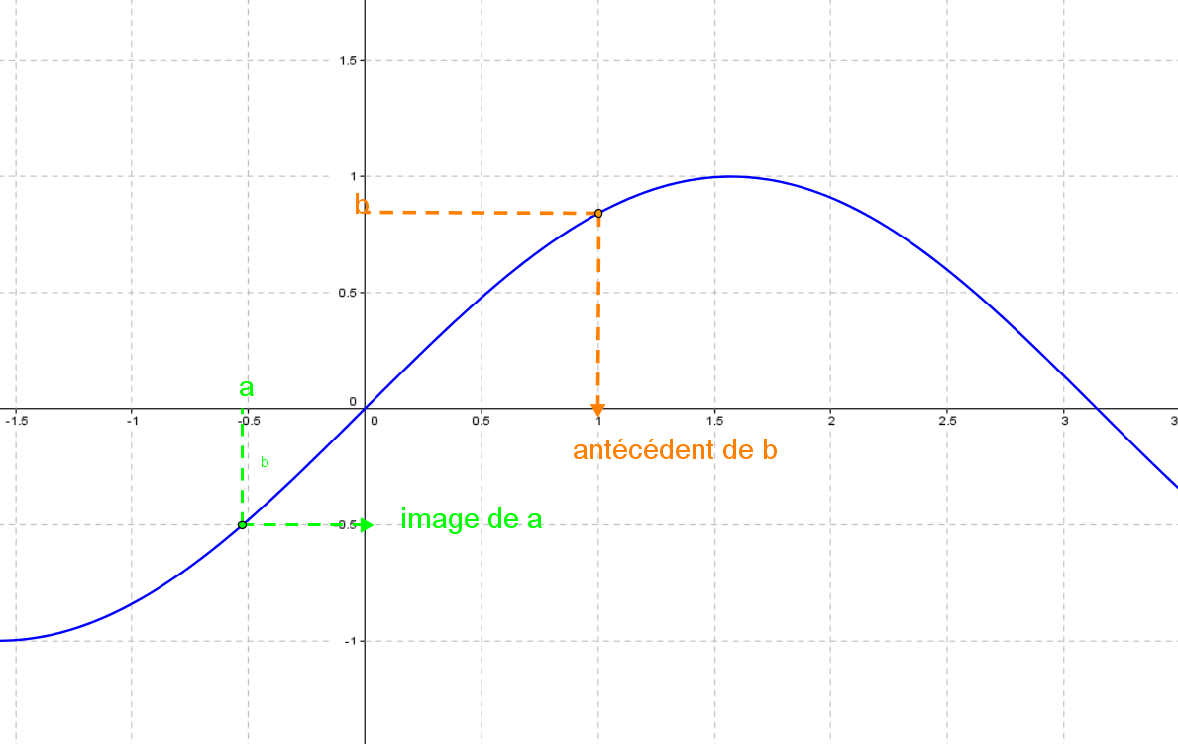
\includegraphics[scale=0.5]{./img/voc}}
\end{myillus}

\section{Fonctions de référence}

\subsection{Fonction carré}

\begin{mydef}
	La \kw{fonction carré} est définie par $x \mapsto x^2$.
\end{mydef}
\begin{myprops}
	\begin{itemize}
		\item Elle est définie pour tous les nombres qui existent (sur l'intervalle $\intervOO{- \infty }{+ \infty}$).
		\item Elle est décroissante sur $\intervOF{- \infty}{0}$.
		\item Elle est croissante sur $\intervFO{0}{+ \infty}$.
	\end{itemize}
	
\end{myprops}

\section{Bonus : Figure incomplète (3 points) }

$ABCD$ est un carré qui a été en partie effacé. On veut tracer son symétrique par rapport au point $O$.

\begin{questions}
	\question[1] Sans compléter le carré $ABCD$, construire $A'B'C'D'$, son symétrique par raport à $O$.
	
	\question[2] \'Ecrire un programme de construction pour $A'B'C'D'$.
\end{questions}

\begin{center}
	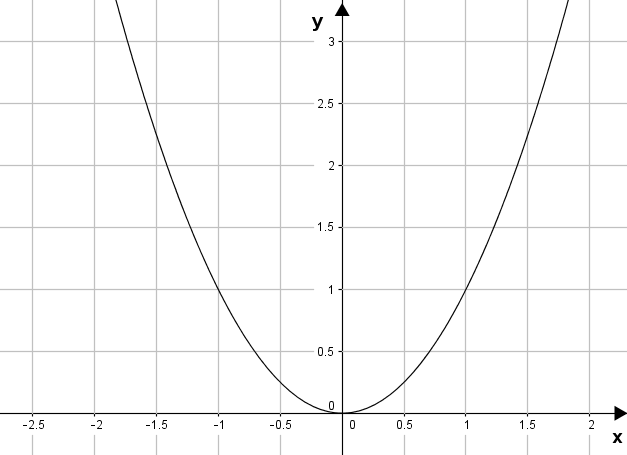
\includegraphics[scale=0.3]{img/carre}
\end{center}

\subsection{Fonction inverse}

\begin{mydef}
	La fonction inverse est définie par $x \mapsto \dfrac{1}{x}$.			
\end{mydef}

\begin{myprops}
	\begin{itemize}
		\item Elle est définie pour tous les nombres qui existent sauf 0, car il n'est pas possible de diviser un nombre par 0 (sur l'intervalle $\intervOO{-\infty}{0} \cup \intervOO{0}{+\infty}$).
		\item Elle est décroissante sur $\intervOO{- \infty}{0}$.
		\item Elle est croissante sur $\intervOO{0}{+ \infty}$. 
	\end{itemize}
\end{myprops}

\begin{myillus}

		Courbe représentative de la fonction $f(x) = \dfrac{1}{x}$ et tableau de variations associé:
	\begin{multicols}{2}

	


	\begin{center}
		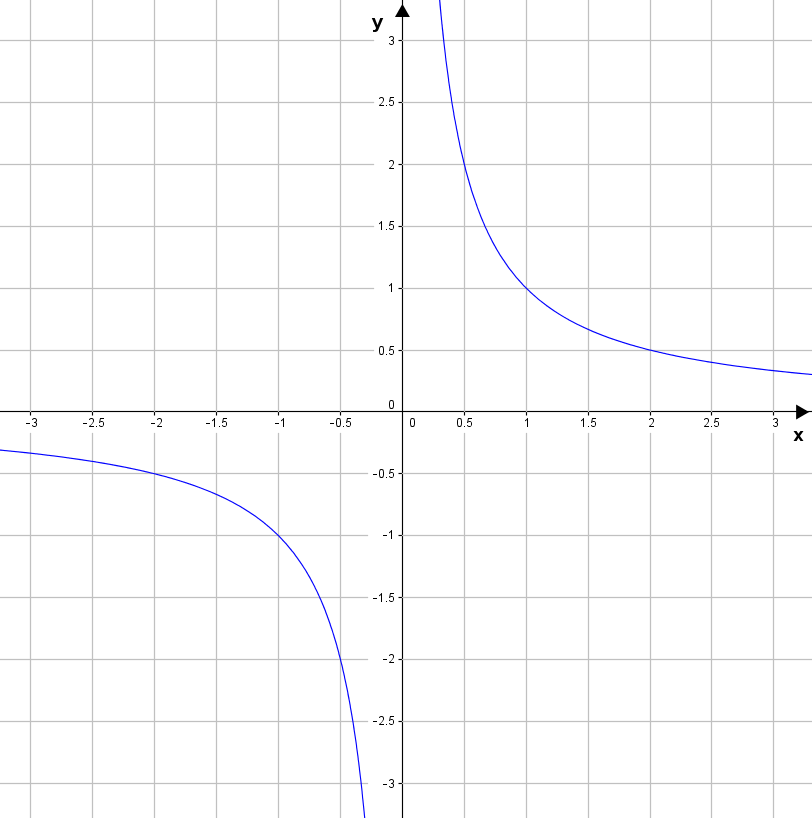
\includegraphics[scale=0.45]{./img/inverse}
	\end{center}
	
	

	\vspace*{1cm}
	\begin{center}
%		\begin{tikzpicture}
%		\tkzTabInit{$x$/1,$f(x)$/2}{$- \infty$,$0$,$+ \infty$}
%		%\tkzTabLine{,-,z,+}
%		\tkzTabVar{+/$+ \infty$,-/$0$,+/$+ \infty$}
%		\end{tikzpicture}	

		\begin{variations}
			x & \mI & & & 0 & & & \pI \\
		\filet
			\m{\dfrac{1}{x}} & \h\ & \d & \ & \bb & \h\ & \d & \ \\				
		\end{variations}
	\end{center}
	\end{multicols}
\end{myillus}
\subsection{Fonction racine}

\begin{mydef}
	La fonction racine carrée est définie par $x \mapsto \sqrt{x}$.			
\end{mydef}

\begin{myprops}
	\begin{itemize}
		\item Elle est définie pour tous les nombres positifs, car on ne peut pas prendre la racine carrée d'un nombre négatif (sur l'intervalle $\intervFO{0}{+\infty}$).
		\item Elle est croissante sur $\intervFO{0}{+ \infty}$. 
	\end{itemize}
\end{myprops}

%\begin{myillus}

		Courbe représentative de la fonction $f(x) = \sqrt{x}$ et tableau de variations associé:
	\begin{multicols}{2}

	


	\begin{center}
		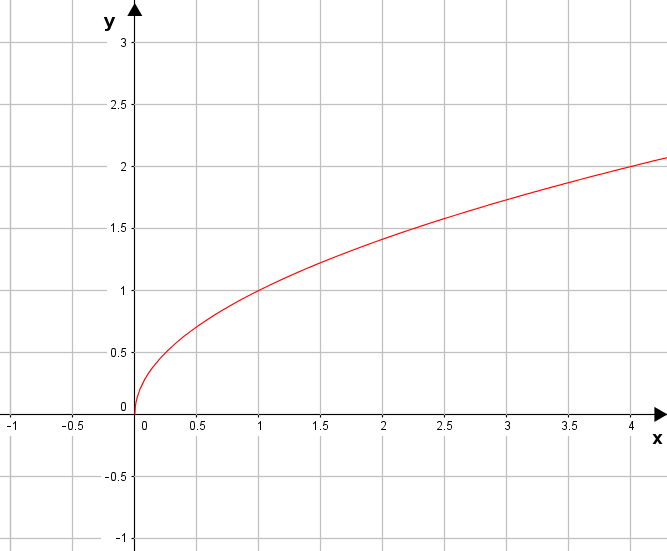
\includegraphics[scale=0.6]{./img/racine}
	\end{center}
	
	

	\vspace*{1cm}
	\begin{center}
%		\begin{tikzpicture}
%		\tkzTabInit{$x$/1,$f(x)$/2}{$- \infty$,$0$,$+ \infty$}
%		%\tkzTabLine{,-,z,+}
%		\tkzTabVar{+/$+ \infty$,-/$0$,+/$+ \infty$}
%		\end{tikzpicture}	

	\begin{variations}
		x & 0 & &  & & \pI \\
		\filet
		\sqrt{x} & & + &  \\				
	\end{variations}

	\vspace*{0.5cm}

		\begin{variations}
			x & & 0 & & \pI \\
		\filet
			\m{\sqrt{x}} & & \ & \c & \h\ \\				
		\end{variations}
	\end{center}
	\end{multicols}
%\end{myillus}
\subsection{Fonction cube}


\begin{mydef}
	La fonction cube est définie par $x \mapsto x^3$.			
\end{mydef}

\begin{myprops}
	\begin{itemize}
		\item Elle est définie pour tous les nombres qui existent (sur l'intervalle $\intervOO{- \infty }{+ \infty}$).
		\item Elle est croissante sur $\intervFO{0}{+ \infty}$. 
	\end{itemize}
\end{myprops}

\begin{myillus}

		Courbe représentative de la fonction $f(x) = x^3$ et tableau de variations associé:
	\begin{multicols}{2}

	


	\begin{center}
		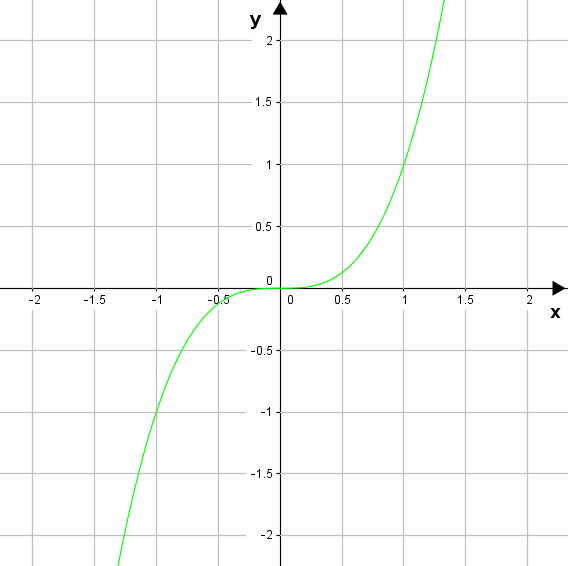
\includegraphics[scale=0.6]{./img/cube}
	\end{center}
	
	

	\vspace*{1cm}
	\begin{center}
%		\begin{tikzpicture}
%		\tkzTabInit{$x$/1,$f(x)$/2}{$- \infty$,$0$,$+ \infty$}
%		%\tkzTabLine{,-,z,+}
%		\tkzTabVar{+/$+ \infty$,-/$0$,+/$+ \infty$}
%		\end{tikzpicture}	

		\begin{variations}
			x & & \mI & & \pI \\
		\filet
			\m{x^3} & & \mI & \c & \h\pI \\				
		\end{variations}
	\end{center}
	\end{multicols}
\end{myillus}
\end{document}